\section{Experimental Results and Discussions}\label{sec:results}
We demonstrate the effectiveness and scalability of random tree search using simulation.
We implemented the random tree search algorithm in C++\footnote{Our tools and data are open-source. Our repository can be accessed at \url{github.com/ahmadyan/Capacitated-Selfish-Replication-Game}} and ran our simulation on a Macbook pro laptop equipped with Core-i7 processor and 16GB of memory.

For case-studies, we use a randomly generated Erdos-Renyi graph $G(n,p)$, where $n$ is the number of players and $p$ is the probability of existence of an edge between two player. We ensured that the graph is connected. The CSR game is for $k$ number of resources in the graph $G$. We executed the random tree search algorithm to find the optimal allocation. The random tree would terminate when the cost function reaches it's maximum at $n\times k$. For each entry point, we repeat the experiments 100 times and reported the mean number of iterations and execition time. To ensure correctness, we checked the number of unsaturated neighborhoods in the graph $G$ to be zero at termination.

%untrivila result No.1
%when we increase the graph size for a fixed p, at the begining the problem gets harder and harder, but after a threshold point (n\p) the problem becomes a lot easier

The hardest example would occur in sparse graphs where $n\times p << k$, where $n$ is the number of players, $k$ is number of resources and $p$ is probability of existence of an edge between two player. $n\times p$ is the expected number of edges between two player. When the expected number of edges is far smaller than the number of resources, the radius of each player substantially increases and as a result, the random tree search has to explore more space to find the optimal allocation.


% two types of results:
% 1. Showing algorithm w.r.t. Number of iterations--> should be linear
% 2. Algorithm w.r.t. its runtime --> O(n^2)

\begin{figure}[htb]
\begin{center}
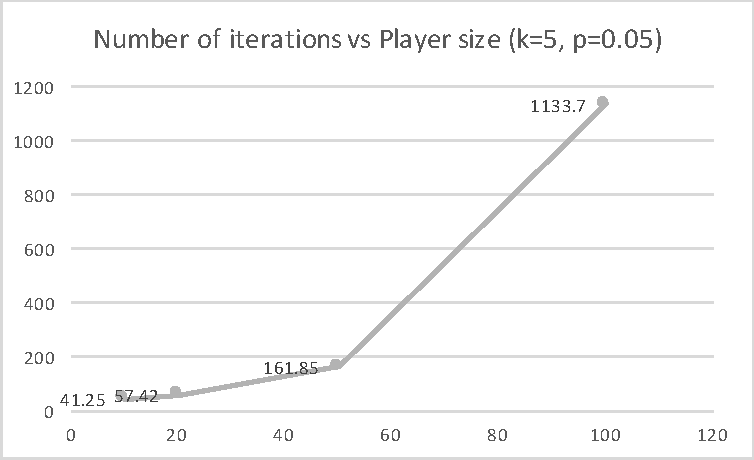
\includegraphics[width=.4\textwidth]{result-1}
\end{center}
\caption{The random tree search algorithm quickly found the opimal allocation for large scale graphs. As we increased the number of players, the number of iterations required for finding the optimal allocation also increased.}
\label{fig:result1}
\end{figure}

\begin{figure}[htb]
\begin{center}
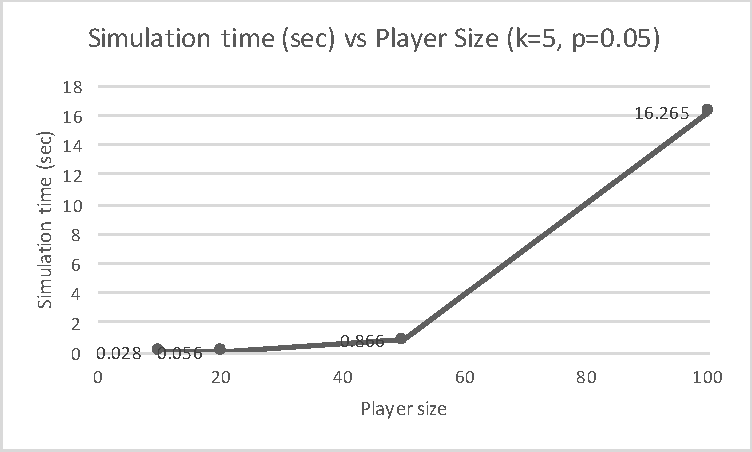
\includegraphics[width=.4\textwidth]{result-2}
\end{center}
\caption{As we increased the number of players, the simulation time required for finding the optimal allocation also increased. The simulation time was linearly corrolated with number of iterations.}
\label{fig:result2}
\end{figure}

\begin{figure}[htb]
\begin{center}
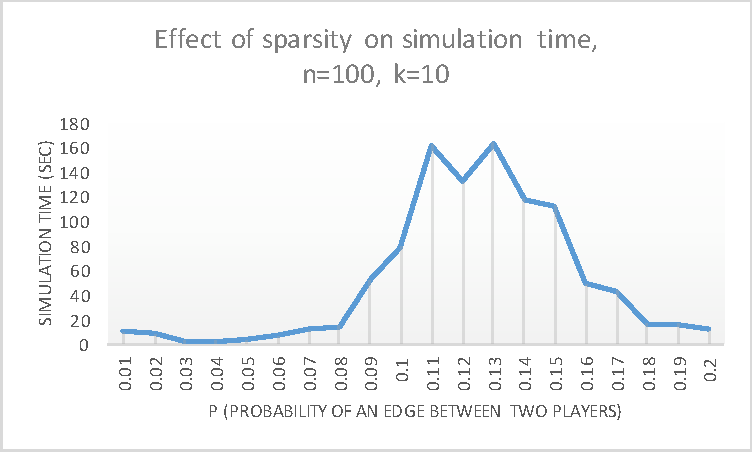
\includegraphics[width=.4\textwidth]{result-3}
\end{center}
\caption{When the graph was very sparse or very dense, the random tree quickly searched the state space and found the optimal allocation. However when the number of resources is roughtly $p\times n$, the search becames more complicated. The random tree stil quickly found the optimal allocation in less 4500 iterations on average. }
\label{fig:result3}
\end{figure}

\begin{figure}[htb]
\begin{center}
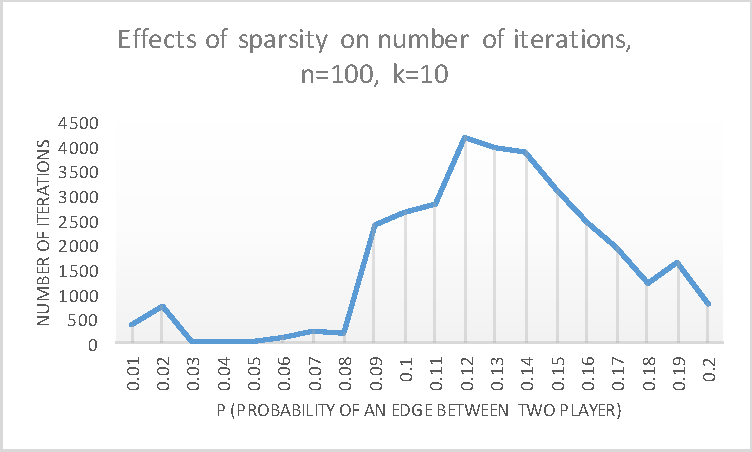
\includegraphics[width=.4\textwidth]{result-4}
\end{center}
\caption{the runtime for the random tree algorithm is linearly corrolated with the number of iterations. When the graph was very sparse or very dense, the random tree quickly searched the state space and found the optimal allocation. However when the number of resources is roughtly $p\times n$, the search becames more complicated. The random tree stil quickly found the optimal allocation in less than 3 minutes.}
\label{fig:result4}
\end{figure}
